\chapter{Le moteur asynchrone}
\section{Principe de fonctionnement}
	\begin{wrapfigure}[10]{l}{4cm}
	\vspace{-5mm}
	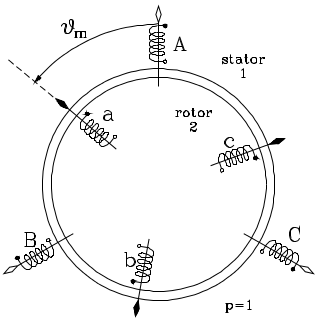
\includegraphics[scale=0.34]{ch5/image1.png}
	\captionof{figure}{ }
	\end{wrapfigure}
Alimentons les phases du stator\footnote{Analogue à celui d'une MS, Cf. ch7.} 
par une source de tension triphasée équilibrée d'ordre direct. Le rotor, lui, 
n'est relié à \textbf{aucune} source de tension (en fonctionnement normal, on 
parle de court-circuit) : il est fermé sur lui même. 
Le couple moteur résultera d'un champ tournant et on peut montrer que la vitesse 
de rotation du rotor $\Omega_r$ ne vaut jamais la vitesse de rotation du 
champ tournant statorique $\Omega_s$ ; \textbf{asynchrone}.\\

Ci-contre, $\vartheta_m$ représente l'angle entre le rotor et le stator. 


\section{Champs fixes et champs tournant}
	\subsection{Champ fixe}
	Comme pour la MCC, l'inducteur est dans le stator. Si la répartition de 
	l'induction est sinusoïdale dans l'entrefer, définissons le vecteur 
	spatial fixe $\vec{B}$ d'amplitude $B^M$ vaut le maximum d'induction, 
	c'est-à-dire l'orientation NS. L'induction au point $X$ repéré par la 
	coordonnée angulaire $\beta_m$ vaut
	\begin{equation}
	\begin{array}{ll}
	B_X &= B^M\cos(p\beta_m)\\
	&= B^M\cos\beta
	\end{array}
	\end{equation}
	\begin{center}
	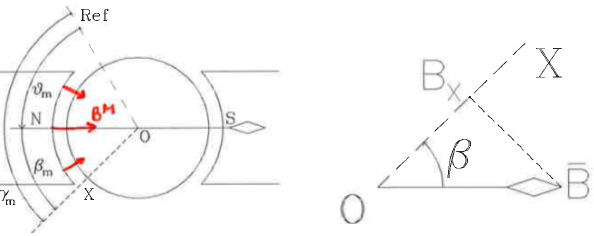
\includegraphics[scale=0.34]{ch5/image2.png}
	\captionof{figure}{ }
	\end{center}
	On multiplie l'angle par $p$ pour avoir l'angle électrique : $\beta_m = 
	\gamma_m-\vartheta_m$. Si $\beta_M \neq f(t)$, l'induction est constante 
	en chaque $X$. On peut alors obtenir la valeur de $B$ en $X$ décalé de 
	$\beta_M$ par rapport à l'axe NS par projection de $\vec{B}$ sur un axe 
	décallé $\beta = p\beta_m$.
	\newpage
	
	\subsection{Champ tournant - Conventions}
	\begin{wrapfigure}[11]{l}{4cm}
%	\vspace{-5mm}
	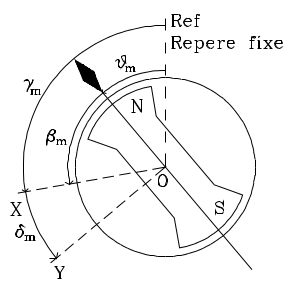
\includegraphics[scale=0.38]{ch5/image3.png}
	\captionof{figure}{ }
	\end{wrapfigure}
	Cette fois-ci, on définit un vecteur spatial $\vec{B}$ qui n'est plus fixe 
	mais \textbf{tournant} amenant la notion de champ sinusoïdal tournant. Par 
	contre le rotor voit un champ fixe, mais sinusoïdal dans l'espace. Notons 
	\begin{itemize}
	\item[$\bullet$] Le sens positif de rotation est le sens trigo.
	\item[$\bullet$] $\gamma_m$ repère $X$ par rapport à un axe statorique 
	fixe : coordonnée statorique.
	\item[$\bullet$] $\beta_m$ repère $X$ par rapport à l'axe $N$ de l'inducteur :
	coordonnée rotorique
	\item[$\bullet$] $\beta_m$ repère l'axe $N$ de l'inducteur par rapport à 
	l'axe statorique de référence.
	\item[$\bullet$] Induction $N \rightarrow S$ est positive.		
	\end{itemize}
	
	
	\subsection{Induction en un point fixe $X$}
	Comme précédemment, si la répartition spatiale de l'induction est sinusoïdale, 
	sa valeur en $X$ vaut 
	\begin{equation}
	B_X = B^M\cos(p\beta_m) = B^M\cos\beta
	\end{equation}
	sauf qu'ici, $\beta_m \neq\ cste$. Si le rotor tourne à vitesse constante 
	$\Omega_r$ :
	\begin{equation}
	\theta_m = \Omega_rt + \theta_{m0}\quad \text{où } \theta_{m0}\ \text{ est 
	la position du rotor en $t=0$}
	\end{equation}
	On a donc
	\begin{equation}
	\theta = p\theta_m = p\Omega_rt + p\theta_{m0} = \omega t +\theta_0
	\end{equation}
	où $\omega = p\Omega_r, \theta_0=p\theta_{m0}$. Jouons avec les phaseurs 
	et nos deux angles $\theta, \gamma$ défini ci-dessus\footnote{Pq $-\gamma$?} :
	\begin{equation}
	\begin{array}{lll}
	B_X &= \Re(\vec{B}.\vec{1_x}^*) &= \Re(B^M\ e^{j(\theta-\gamma)})\\
	&= \Re(B^M\ e^{j(\omega t + \theta_0-\gamma)}) &= B^M\cos(\omega t+\theta_0
	-\gamma)
	\end{array}
	\end{equation}
	Le champ $B_x$ varie donc sinusoïdalement dans le temps. On peut encore 
	l'écrire 
	\begin{equation}
	B_X = \Re(B^M\ e^{j(\theta_0-\gamma)}\ e^{j\omega t}) \equiv \Re(\underline{B}
	\sqrt{2}\ e^{j\omega t})
	\end{equation}
	avec 
	\begin{equation}
	\underline{B} = \dfrac{B^M}{\sqrt{2}}\ e^{j(\theta_0-\gamma)}
	\end{equation}
	

	Un observateur rotorique verra une répartition spatiale de l'induction alors 
	qu'un observateur statorique (fixe) voit passer un champ tournant. Un 
	observateur statorique placé à un autre endroit voit le même champ tournant, 
	de même amplitude mais déphasé. L'illustration ci-dessus montre deux moyens 
	d'obtenir $B_X$ et $B_Y$.
	\begin{center}
	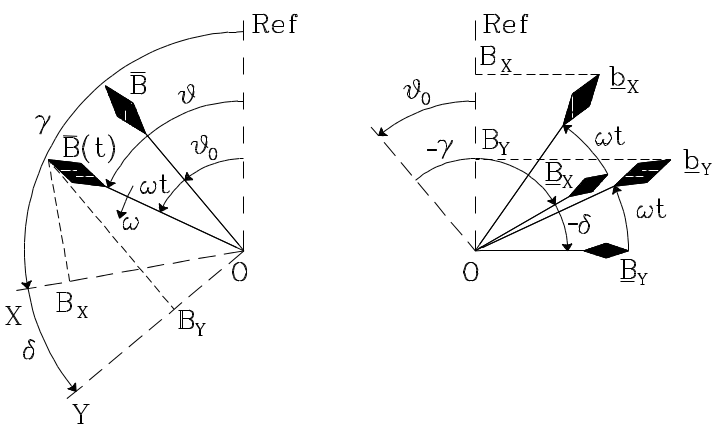
\includegraphics[scale=0.34]{ch5/image4.png}
	\captionof{figure}{Ces deux représentations donnent les mêmes infos : l'une est 
	un champ qui tourne "physiquement" et l'autre est repris en phaseurs.}
	\end{center}
	

\section{Les f.e.m. engendrées dans les enroulements ouverts}
	\subsection{Étoiles des encoches}
		\begin{wrapfigure}[11]{l}{10cm}
	\vspace{-5mm}
	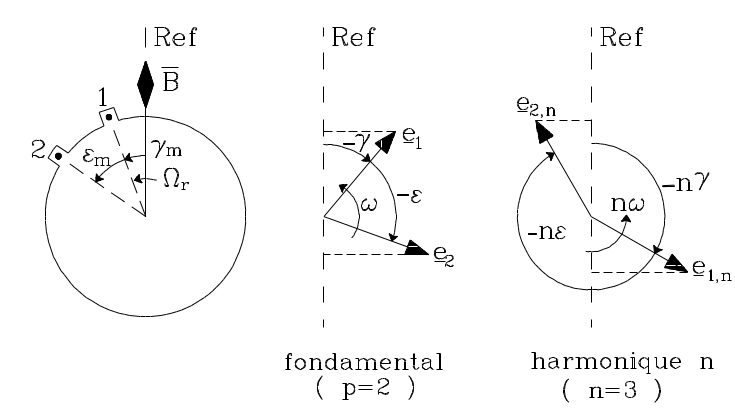
\includegraphics[scale=0.38]{ch5/image5.png}
	\captionof{figure}{ }
	\end{wrapfigure}
	Le calcule des phaseurs de tension pour un conducteur 1, décalé de 
	$\gamma_m$ s'obtient via $e= Blv$.\\
			1 et 2 sont deux conducteurs fixes dans des encoches. $\Omega_r$ 
	est la vitesse de rotation mécanique. Comme $e=Blv$, la tension $\propto B \rightarrow$ 
	les phaseurs de $B$ et $e$ ont la même direction. Le $-\epsilon$ signifie que $e_2$ 
	est en retard par rapport à $e_1$.\\
	

	\subsection{Étoiles des bobines - Raccourcissement du pas}
	Soit une spire composée d'un conducteur aller 1 et retour 1'. Si les spires sont 
	diamétrales (électriquement opposé, $\angle 11' = \pi/p$), la tension à ses bornes 
	est simple : $e_{(1)} = e_1-e_{1'}$.
	\begin{center}
	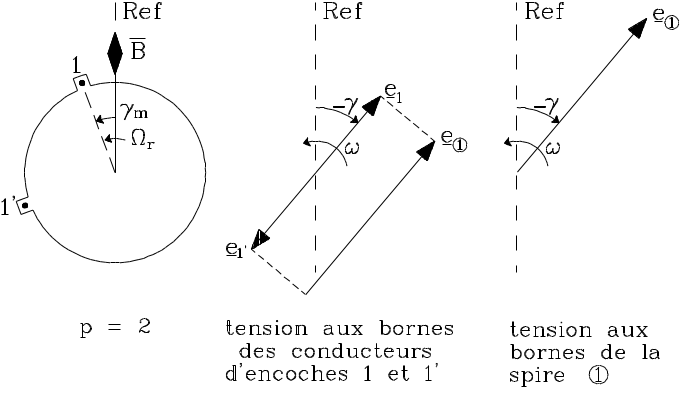
\includegraphics[scale=0.38]{ch5/image6.png}
	\captionof{figure}{ }
	\end{center}
	
	\newpage	
	Si la spire (11') n'est \textbf{pas} diamétrale, les choses changent. Considérons 
	le conducteur 1" tel que la spore 11" soit diamétrale : la tension en 1' est 
	déphasée de $np\delta m=n\delta$ par rapport à celle en 1" valant l'opposé de celle 
	en 1. La f.e.m. $e_{(1)}=e_1-e_{1'}$ est décalée de $n\delta/2$ par rapport à $e_1$.\\
	
	\begin{wrapfigure}[11]{l}{9cm}
	\vspace{-5mm}
	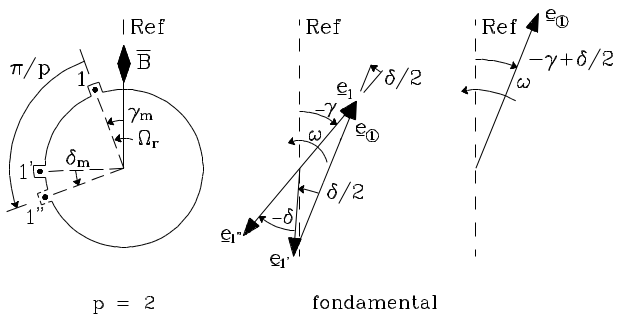
\includegraphics[scale=0.38]{ch5/image7.png}
	\captionof{figure}{ }
	\end{wrapfigure}
	Dû au raccourcissement du pas $\delta_m$, l'amplitude est inférieur à $2*e_1$. La 
	phase est donc identique à celle d'une spire \textbf{diamétrale} de même axe que 
	la spire 11'. Cette spire diamétrale équivalente est décalée d'un angle mécanique 
	négatif $-\delta_m/2$ par rapport à 1 et d'un angle mécanique positif $\delta_m/2$ 
	par rapport à 1'. On peut alors calculer la f.e.m. dans la spire réelle en multipliant 
	la f.e.m. de la spire diamétrale équivalente par le \textbf{facteur de raccourcissement 
	de pas }
	\begin{equation}
	k_R = \cos\dfrac{n\delta}{2}=\cos\dfrac{np\delta_m}{2}
	\end{equation}
	où $n$ est le numéro de l'harmonique.
	
	\subsection{Étalage des encoches}
	\begin{wrapfigure}[11]{r}{9cm}
	\vspace{-8mm}
	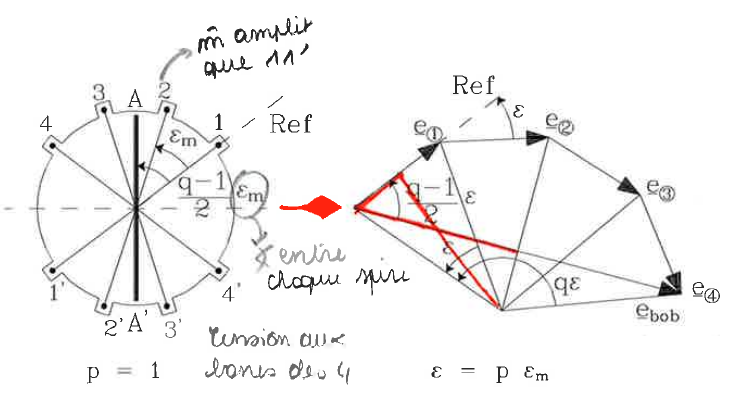
\includegraphics[scale=0.38]{ch5/image8.png}
	\captionof{figure}{ }
	\end{wrapfigure}
	On considère maintenant $q$ spires diamétrales en séries décalée d'un angle mécanique
	$\epsilon_m$ l'une par rapport à l'autre. Toutes les spires (22',33',\dots) ont la 
	même amplitude que 11'. Vu qu'elles sont en série, on prend la tension aux bornes des 
	(ici) quatre spires, les tensions vont s'additionner mais la tension totale ne vaudra 
	pas quatre fois celle de la spire 11' : facteur de diminution. On l'appelle le 
	\textbf{facteur d'étalage} que l'on peut calculer avec la règle des sinus :
	\begin{equation}
	k_E = \dfrac{\sin\left(\dfrac{nq\epsilon}{2}\right)}{q\sin\left(\dfrac{n\epsilon}{2}
	\right)}
	\end{equation}
	
	\subsection{Obliquité des encoches}
	Si les encoches sont \textit{un peu de travers}, l'amplitude de la tension réelle 
	est obtenue en multipliant la tension aux bornes du conducteur par le \textbf{facteur 
	d'obliquité }:
	\begin{equation}
	k_0 = \dfrac{\sin np/2}{np/2}
	\end{equation}
	On peut utiliser cette technique pour supprimer les harmoniques des dentures.
	
	\subsection{Tension aux bornes d'une bobine}
	"\textit{En résumé, la tension aux bornes d'une bobine est obtenue en multipliant la 
	tension aux bornes d'une bobine constituée d'un même nombre de spires diamétrales dont 
	l'axe est celui de la bobine réelle, par le produit des facteurs d'obliquité, d'étalage 
	et de raccourcissement de pas.}"
	
	
\section{Champ magnétique et inductance dans la machine linéaire à entrefer constant}
On cherche à obtenir les coefficients d'inductance propre et mutuelles entre les enroulements 
comme pour le transformateur.

	\subsection{Force magnétomotrice dans une machine à entrefer constant}
		\begin{wrapfigure}[11]{r}{5cm}
	\vspace{-5mm}
	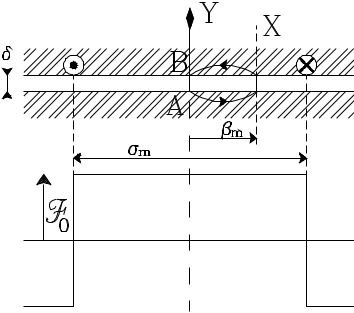
\includegraphics[scale=0.38]{ch5/image9.png}
	\captionof{figure}{ }
	\end{wrapfigure}
	Soit une bobine d'axe $Y$ avec $N_1$ spires confondues. La largueur (angulaire) de 
	ces spires vaut $\sigma_m$. On repère le point $X$ par sa coordonnée $\beta_m$ par 
	rapport à l'axe de la bobine. La différence de potentiel magnétique entre stator 
	et rotor dans l'axe $A-B$ vaut 
	\begin{equation}
	\Delta V_0 = H_{(0)}\delta \equiv \mathcal{F}_0
	\end{equation}
	souvent dit \textit{force magnétomotrice} $\mathcal{F}_0$ par abus de langage. Par 
	convention la f.m.m. au point $X$ ($\mathcal{F}_{(\beta m)}$ désigne la f.m.m. entre 
	les points $A$ et $B$ le long d'un chemin traversant l'entrefer au point $X$. La loi 
	des f.m.m. donne (Ampère)\footnote{??} :
	\begin{equation}
	\begin{array}{ll}
	\mathcal{F}_{(\beta m)} - \mathcal{F}_0 &= 0  \text{ si } |\beta_m|<\sigma_m/2\\
	&= -Ni  \text{ si } |\beta_m|>\sigma_m/2
	\end{array}
	\end{equation}
	Par symétrie, $\mathcal{F}_0 = Ni/2$. Si le fer est parfait et l'entrefer constant, 
	le champ magnétique vaut 
	\begin{equation}
	\begin{array}{ll}
	H_{(\beta m)} &= \dfrac{Ni}{2\delta}\ \text{ si }\ |\beta_m|<\sigma_m/2\\
	&= -\dfrac{Ni}{2\delta}\ \text{ si }\ |\beta_m|>\sigma_m/2
	\end{array}
	\end{equation}
	et l'induction
	\begin{equation}
	B_{(\beta m)} = \mu_0H_{(\beta_m)}
	\end{equation}
	La figure ci-dessous représente l'effet de bobines concentriques à même nombre de 
	spires parcourues par le même courant. On voit que cela ressemble fortement à un 
	beau sinus
	\begin{center}
	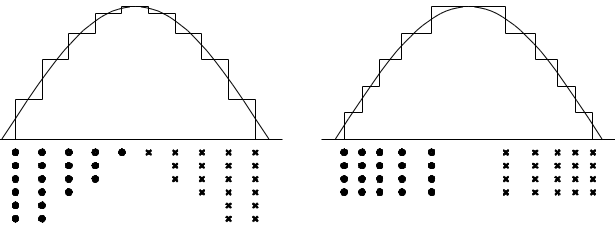
\includegraphics[scale=0.38]{ch5/image10.png}
	\captionof{figure}{ }
	\end{center}
	
	\subsection{Titre beaucoup trop long}
	Pour une sous-section dont il a seulement dit quelque chose ?
	
	\newpage
	\subsection{Facteurs d'étalage, de raccourcissement, d'obliquité}
	\begin{wrapfigure}[8]{l}{9cm}
	\vspace{-5mm}
	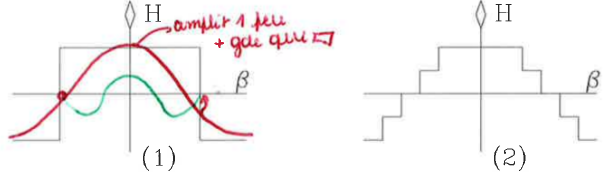
\includegraphics[scale=0.38]{ch5/image11.png}
	\captionof{figure}{ }
	\end{wrapfigure}
	Ci-contre, à gauche quatre spire diamétrales et à droite quatre spires 
	étalées. En configuration étalée, le champ est bien plus sinusoïdal et il peut 
	l'être complètement avec un choix judicieux (hypothèse pour le reste du cursus).\\

	Limité à son fondamental, le champ à pour expression
	\begin{equation}
	H_{(\beta)} = k_Ek_Rk_O\dfrac{N_fi_f}{2\delta p}\dfrac{4}{\pi}\cos\beta
	\end{equation}
	Dans un cas \textit{confondu}, $N_f/p$ représente les spires en dessous de la 
	première paire de pôle. Dans le cas \textit{réparti}, on ne prend plus que le 
	fondamental. Le facteur de "correction rectangle" pour n'obtenir que le fondamental 
	est $4/\pi$. Après, les facteurs d'obliquité, \dots sont présents pour effectuer 
	les différentes corrections.\\
	Pour rendre ça tout smooth, on défini le \textbf{nombre effectif de spires}
	\begin{equation}
	N_{sf} \equiv \dfrac{4}{\pi}k_Ek_Rk_ON_f
	\end{equation}
	Ce nombre de spire donne le même "fondamental". On peut alors écrire
	\begin{equation}
	H_{(\beta)} = \dfrac{N_{sf}i_f}{2\delta p}\cos\beta
	\end{equation}
	On note aussi souvent $k_f=k_ek_Rk_O$ pour rendre ça $e^{\text{smooth}}$.
	
	
	\subsection{Inductance propre d'une bobine dans une machine à entrefer constant}
	\begin{wrapfigure}[8]{l}{5cm}
	\vspace{-8mm}
	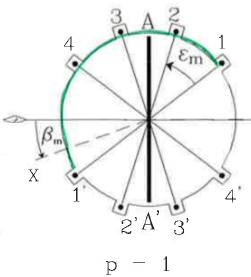
\includegraphics[scale=0.45]{ch5/image12.png}
	\captionof{figure}{ }
	\end{wrapfigure}
	Soit $q$ spires décalées de $\epsilon_m$ l'une de l'autre. Avec le courant $i_f$, 
	le \textbf{fondamental} du champ vaut au point $X$ de coordonnée $\beta_m$ :
	\begin{equation}
	H_{(\beta)} = k_E\dfrac{N_fi_f}{2\delta p}\dfrac{4}{\pi}\cos\beta
	\end{equation}
	L'induction se déduit directement : $B_{(\beta)} = \mu_0H_{(\beta)}$. Le flux 
	coupé par la spire (1) vaut \\
	\ \\
	
	\begin{equation}
	\Phi_{(1)} = \int_{-\frac{\pi}{2p}-\frac{q-1}{2}\epsilon_m}^{\frac{\pi}{2p}-
	\frac{q-1}{2}\epsilon_m} B_{(\beta_m)} lRd\beta_m = \dfrac{\mu_0lR}{p^2\delta}
	\left(\dfrac{4}{\pi}k_EN_f\right)i_f\cos\dfrac{q-1}{2}\epsilon
	\end{equation}
	On peut voir $\Phi_{(1)}$ comme la valeur de la projection de la spire du flux
	$\Phi_\perp$ coupé par une spire identique mais dont l'axe serait celui de la 
	bobine \textbf{ou} le flux coupé par la spire diamétrale après qu'on ai 
	inversé les axes de la bobine et de la spire.
	\begin{equation}
	"\ \Phi_\perp \cos\dfrac{q-1}{2}\epsilon\ "
	\end{equation}
	
	\begin{center}
	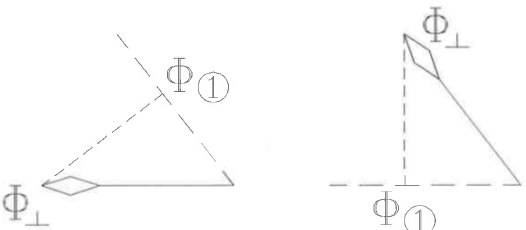
\includegraphics[scale=0.45]{ch5/image13.png}
	\captionof{figure}{ }
	\end{center}
	On a alors
	\begin{equation}
	\Phi_\perp = \dfrac{\mu_0lR}{p^2\delta}\left(\dfrac{4}{\pi}k_EN_f\right)i_f
	\end{equation}
	Ceci est le flux dans une des spires. L'avantage c'est que maintenant on peut 
	tout sommer brutalement, même les spires qui ne sont pas dans la même direction!\\
	
	\begin{wrapfigure}[7]{r}{5cm}
	\vspace{-8mm}
	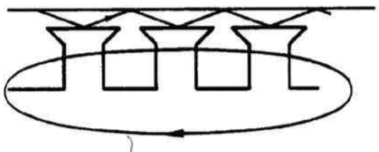
\includegraphics[scale=0.45]{ch5/image14.png}
	\captionof{figure}{ }
	\end{wrapfigure}
	Le flux totalisé pour $N_f/p$ spires d'une paire de pôles s'obtient comme on 
	l'avait fait avant, en tenant compte de $k_E$ :
	\begin{equation}
	\Psi_{\text{2 pôles}} = k_E\dfrac{N_f}{p}\Phi_\perp = \dfrac{1}{p}(k_EN_f)
	\dfrac{\mu_0}{p^2\delta}lR\left(\dfrac{4}{\pi}k_EN_f\right)i_f
	\end{equation}
	Et donc pour $p$ paires de pôles :
	\begin{equation}
	\Psi = \left(\dfrac{4}{\pi}k_EN_f\right)^2\dfrac{\pi}{4}\dfrac{\mu_0lR}{p^2\delta}
	i_f
	\end{equation}
	On peut faire le même raisonnement avec $k_O$ et $k_R$. On obtiendrait alors :
	\begin{equation}
	\Psi = i_fN_{sf}^2\mathcal{P}_m
	\end{equation}
	où $N_{sf}$ est le nombre effectif de spires et $\mathcal{P}_m$ est la perméance 
	du circuit magnétique (mise en série de $2p$ entrefers). Ceci ne concerne que 
	la flux dans l’entrefer (flux utile, commun) sans le traverser (le flux reste 
	dans le stator). \\
	On en déduit l'inductance \textbf{linéaire} de la bobine pour le fondamental du 
	champ
	\begin{equation}
	L_f = l_f + N_{sf}^2\mathcal{P}_m
	\end{equation}
	Expression semblables à celle des transfo et non-influencée par la position du
	rotor.
	
	
	\subsection{Inductance mutuelle entre une bobine statorique et une bobine rotorique 
	dans une machine à entrefer constant}
	Soit un enroulement statorique $A$ et un rotorique $f$ dont les axes sont 
	décalés de $\chi$. Il faut suivre un raisonnement similaire au chapitre précédent. 
	Le flux coupé par une spire diamétrale d'axe $f$ pour un courant statorique $i_a$ 
	vaut
	\begin{equation}
	\Phi_\chi = \Phi_\perp\cos\chi
	\end{equation}
	Rebelote (après quelques calculs) :
	\begin{equation}
	\Psi_{fA} = l_fN_f\Phi_\chi =  i_AN_{sf}N_{sA}\mathcal{P}_m\cos\chi
	\end{equation}
	On trouve que le flux d'entrefer (commun) créé et 	coupé par $A$ vaut 
	\begin{equation}
	\Psi_{AA} = i_AN_{sA}^2\mathcal{P}_m
	\end{equation}
	L'expression de la mutuelle entre les deux enroulements est alors
	\begin{equation}
	M_{fA} = N_{sf}N_{sA}\mathcal{P}_m\cos\chi
	\end{equation}
	où les $N_i$ représentent les nombres de spires rotor/stator, $\mathcal{P}_m$ 
	est nécessaire car les flux traversent l'entrefer, $\chi$ est l'angle 
	électrique si l'on a $p$ paires de pôles et la présence du $\cos$ intervient 
	alors lorsque ceux-ci ne sont pas alignés.
	
	\subsection{Inductance mutuelle entre deux bobines statoriques dans une machine 
	à entrefer constant}	
	On peut déduire cette expression dans un systèmes triphasé avec la formule 
	précédente, si $\chi=2\pi/3$. Il faut cependant rajouter un terme supplémentaire 
	provenant du flux de dispersion d'une phase qui, même s'il ne traverse pas 
	l'entrefer, arrive à l'autre phase :
	\begin{equation}
	M_{AB} = l_A'+N_1^2\mathcal{P}_m\cos\dfrac{2\pi}{3} = l_A'-\dfrac{1}{2}N_1^2
	\mathcal{P}_m
	\end{equation}
	On obtient des expressions semblables pour le rotor.
	
	\subsection{Matrice des coefficients d'inductance pour une machine linéaire à 
	entrefer constant comportant 3 enroulement $ABC$ au stator et 3 enroulement 
	$abc$ au rotor}
	\begin{wrapfigure}[11]{r}{4cm}
	\vspace{-8mm}
	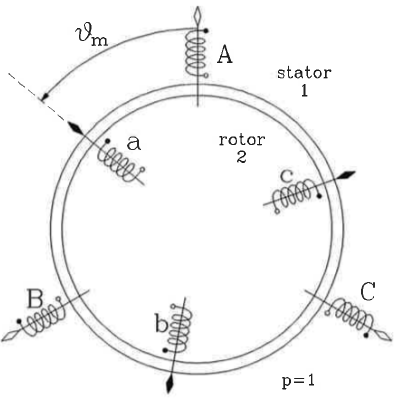
\includegraphics[scale=0.3]{ch5/image15.png}
	\captionof{figure}{ }
	\end{wrapfigure}
	La page 5.28 reprends la définition des différentes phases, il faut ensuite 
	tout injecter dans une matrice beaucoup trop grande pour que je la  mette ici. 
	Rien de compliquer, c'est vraiment appliquer les formules trouvées plus haut.\\
	
	A l'examen, on peut demander un moyen de calculer les inductances via différents 
	nombre de spires effectives et des facteurs d'états,\dots\\
	
	On obtient une belle matrice d'inductances qui permet de calculer tous les flux 
	en fonction des courants (et pleins de paramètres, évidemment). Rappelons que 
	pour avoir un sens, il ne faut pas prendre en tête les  hypothèses suivantes:
	\begin{enumerate}
	\item Harmoniques spatiaux de $B,H$ et de la f.m.m. négligés
	\item Entrefer constant
	\item Non-linéarités magnétiques négligées
	\end{enumerate}
	De plus, ces expression sont valables en valeurs \textbf{instantanées}.
	
	
	\newpage
\section{Champs pulsant et champs tournants}
	
	
	
	
	
	
	
	
	
	
	